% =====================================================================
%  MCMP117 -- Fundamentals of Operating Systems
%  Week 12 Course Notes: Text Processing, Redirection & Pipes
%  Compile with XeLaTeX (twice):  xelatex MCMP117_Week12_Notes.tex
%  Needs ./figures/ and the ../code/ folder.
% =====================================================================
\documentclass[11pt,a4paper]{article}
\newcommand{\weeknum}{12}
% ---------- Page & fonts ---------------------------------------------
\usepackage[a4paper,margin=2.3cm,headheight=15pt]{geometry}
\usepackage{fontspec}
\IfFontExistsTF{Calibri}{\setmainfont{Calibri}}{\setmainfont{Carlito}}
\IfFontExistsTF{Cambria}{\newfontfamily\headfont{Cambria}}{\newfontfamily\headfont{Caladea}}
\IfFontExistsTF{Consolas}{\setmonofont[Scale=0.95]{Consolas}}{\setmonofont[Scale=0.88]{DejaVu Sans Mono}}
\usepackage{amsmath,amssymb}
\usepackage{microtype}
\linespread{1.12}
\setlength{\parskip}{0.55em}
\setlength{\parindent}{0pt}

% ---------- Colours (course design system) ----------------------------
\usepackage{xcolor}
\definecolor{dark}{HTML}{212121}
\definecolor{charcoal}{HTML}{36454F}
\definecolor{slate}{HTML}{50808E}
\definecolor{mint}{HTML}{02C39A}
\definecolor{mintdeep}{HTML}{028090}
\definecolor{light}{HTML}{F2F2F2}
\definecolor{muted}{HTML}{6B7679}

% ---------- Packages ---------------------------------------------------
\usepackage{graphicx}
\usepackage{float}
\usepackage{needspace}
\graphicspath{{figures/}}
\usepackage[font=small,labelfont={bf,color=mintdeep},justification=centering]{caption}
\usepackage{booktabs,longtable,array,tabularx}
\usepackage{enumitem}
\setlist{itemsep=0.25em,topsep=0.3em}
\usepackage{tikz}
\usetikzlibrary{arrows.meta,positioning,calc,shapes.geometric}
\usepackage{pgfplots}
\pgfplotsset{compat=1.17}
\usepackage[most]{tcolorbox}
\usepackage{titlesec}
\usepackage{fancyhdr}
\usepackage{xurl}
\usepackage[colorlinks=true,linkcolor=mintdeep,urlcolor=mintdeep,citecolor=mintdeep]{hyperref}

% ---------- Headings ----------------------------------------------------
\titleformat{\section}{\headfont\Large\bfseries\color{charcoal}}{\color{mint}\thesection}{0.7em}{}
\titleformat{\subsection}{\headfont\large\bfseries\color{charcoal}}{\color{mintdeep}\thesubsection}{0.6em}{}
\titleformat{\subsubsection}{\headfont\normalsize\bfseries\color{mintdeep}}{}{0em}{}
\titlespacing*{\section}{0pt}{1.6em}{0.6em}
\titlespacing*{\subsection}{0pt}{1.2em}{0.4em}

% ---------- Header / footer -----------------------------------------------
\pagestyle{fancy}
\fancyhf{}
\fancyhead[L]{\small\color{muted}MCMP117 --- Fundamentals of Operating Systems}
\fancyhead[R]{\small\color{muted}Week \weeknum{} Notes}
\fancyfoot[C]{\small\color{muted}\thepage}
\renewcommand{\headrulewidth}{0pt}

% ---------- Boxes ---------------------------------------------------------
\newtcolorbox{keyidea}[1][Key idea]{enhanced,breakable,colback=charcoal,colframe=charcoal,
  coltext=white,fonttitle=\headfont\bfseries\color{mint},title={#1},
  attach title to upper={\par\smallskip},boxrule=0pt,arc=3pt,left=10pt,right=10pt,top=8pt,bottom=8pt}
\newtcolorbox{example}[1][Worked example]{enhanced,colback=light,colframe=light,
  fonttitle=\headfont\bfseries\color{mintdeep},title={#1},attach title to upper={\par\smallskip},
  boxrule=0pt,arc=3pt,left=10pt,right=10pt,top=8pt,bottom=8pt}
\newtcolorbox{tryit}[1][Try it yourself]{enhanced,breakable,colback=white,colframe=mint,
  fonttitle=\headfont\bfseries\color{mintdeep},title={#1},attach title to upper={\par\smallskip},
  boxrule=0.8pt,arc=3pt,left=10pt,right=10pt,top=8pt,bottom=8pt}
\newtcolorbox{histnote}[1][Historical note]{enhanced,breakable,colback=white,colframe=slate!40,
  fonttitle=\headfont\bfseries\color{slate},title={#1},attach title to upper={\par\smallskip},
  boxrule=0.5pt,arc=3pt,left=10pt,right=10pt,top=8pt,bottom=8pt,fontupper=\small}

% Photo helper: fits image inside a box, never distorted (keepaspectratio)
\newcommand{\photo}[3]{\includegraphics[width=#1,height=#2,keepaspectratio]{#3}}

\newcommand{\term}[1]{\textbf{\color{mintdeep}#1}}
\newcommand{\cmd}[1]{\texttt{#1}}


% ---------- Code listings ----------------------------------------------------
\usepackage{listings}
\lstdefinestyle{course}{
  basicstyle=\ttfamily\small, columns=fullflexible, keepspaces=true,
  backgroundcolor=\color{dark}, rulecolor=\color{dark}, frame=single, framesep=6pt,
  xleftmargin=8pt, xrightmargin=8pt, aboveskip=0.8em, belowskip=0.6em,
  basicstyle=\ttfamily\small\color{light},
  keywordstyle=\color{mint}\bfseries, commentstyle=\color{white!60}\itshape,
  stringstyle=\color{orange!70!yellow}, numberstyle=\tiny\color{muted},
  numbers=left, numbersep=10pt, showstringspaces=false, breaklines=true,
  tabsize=4, upquote=true}
\lstdefinestyle{term}{style=course, numbers=none, keywordstyle=\color{light},
  commentstyle=\color{white!60}, stringstyle=\color{light}}
\lstset{style=course,language=C}
\usepackage{textcomp}

\begin{document}
% ============================ Week 12 body ============================
% terminal sessions are long in a Linux week: print them one size smaller
\setlength{\emergencystretch}{3em}
\lstdefinestyle{term}{style=course, numbers=none, keywordstyle=\color{light},
  commentstyle=\color{white!60}, stringstyle=\color{light}, basicstyle=\ttfamily\footnotesize\color{light}}
\thispagestyle{empty}
\begin{tcolorbox}[enhanced,colback=dark,colframe=dark,arc=0pt,boxrule=0pt,
  left=18pt,right=18pt,top=20pt,bottom=20pt,coltext=white]
{\small\color{mint}\textsc{MCMP117 \,·\, Week 12 \,·\, Course Notes}}\par\medskip
{\headfont\fontsize{26}{30}\selectfont\bfseries Fundamentals of Operating Systems}\par\medskip
{\large Text Processing, Redirection \& Pipes}\par\smallskip
{\small\itshape\color{white!70} Small programs, connected by the kernel, answer real questions about real data.}
\end{tcolorbox}

\vspace{0.4em}
{\small
\textbf{Instructor:} Asst.\ Prof.\ Dr.\ (Ph.D.) Hasan Oğuz\\
Head of the Electronical Communication Technology Programme, Vocational School\\
Istanbul Okan University\par}

\vspace{0.8em}
\begin{keyidea}[What you should be able to do after this week]
\begin{enumerate}[leftmargin=1.4em]
  \item Explain standard input, standard output and standard error as the file descriptors $0$, $1$ and $2$, and connect them to the \cmd{write(1, \dots)} system call of Weeks~2--3.
  \item Use the redirections \cmd{>}, \cmd{>>}, \cmd{<}, \cmd{2>}, \cmd{2>\&1}, \cmd{\&>} and \cmd{/dev/null}, and predict the effect of their order.
  \item Explain how the shell implements redirection and pipes with \cmd{fork()}, \cmd{open()}, \cmd{pipe()}, \cmd{dup2()} and \cmd{exec()}, and read the corresponding \cmd{strace} output.
  \item Use the filters \cmd{grep} (with \cmd{-i -n -v -c -w -r} and simple regular expressions), \cmd{sort}, \cmd{uniq}, \cmd{cut}, \cmd{wc}, \cmd{tr}, \cmd{head}, \cmd{tail} and \cmd{tee}.
  \item Search the directory tree with \cmd{find} and act on the results with \cmd{-exec} or \cmd{xargs}.
  \item Answer questions about log files and CSV data with one-line pipelines, built one stage at a time.
\end{enumerate}
\end{keyidea}

\setcounter{tocdepth}{1}
\tableofcontents

% =====================================================================
\section{From Week 11 to Week 12}

Last week we looked at files from the outside: who owns them (\cmd{id}, \texttt{/etc/passwd}), what the mode string \texttt{-rwxr-x---} means, and how \cmd{chmod} changes it, symbolically (\cmd{u+x}) or in octal ($754$: $7 = 4+2+1$ for the owner, $5 = 4+1$ for the group, $4$ for others). This week we look \emph{inside} files. Linux keeps almost everything --- configuration, logs, data exports --- as plain text, one record per line. A small set of tools that read lines, filter them and write lines can therefore answer a surprising range of questions. The glue that connects these tools is provided by the operating system: \term{redirection} and \term{pipes}. Both rest on one idea you have already met, the \term{file descriptor}.

\paragraph{How to follow these notes.} All examples run in the practice folder \texttt{\textasciitilde/lab}. Re-create it before you start, so that your files are identical to ours:
\begin{lstlisting}[style=term]
$ bash mcmp117_lab_setup.sh
$ cd ~/lab
\end{lstlisting}
Every session shown here is real output, captured as an ordinary user with the scripts \texttt{code/demo\_*.sh} (the output files are \texttt{code/out\_*.txt}). On your machine, dates, process numbers (PIDs), terminal names (\texttt{/dev/pts/1}) and user names will differ. The order of \cmd{ls} and \cmd{sort} output can also depend on the \emph{locale} (language settings); we used \cmd{LC\_ALL=C.UTF-8}, in which upper-case letters sort before lower-case ones. Type \cmd{export LC\_ALL=C.UTF-8} if your results are ordered differently.

% =====================================================================
\section{Standard Streams and File Descriptors}
\label{sec:streams}

\subsection{Three open files from birth}

In Week~7 we saw that a process does not refer to an open file by its name but by a small integer, the \term{file descriptor} (fd): an index into the process's \emph{per-process open-file table}. When the shell starts a program, three descriptors are already open:

\begin{center}
\renewcommand{\arraystretch}{1.25}
\begin{tabular}{@{}clll@{}}
\toprule
\textbf{fd} & \textbf{Name} & \textbf{Used for} & \textbf{Default in a terminal}\\
\midrule
$0$ & standard input (stdin) & data the program reads & the keyboard\\
$1$ & standard output (stdout) & normal results & the terminal screen\\
$2$ & standard error (stderr) & error and diagnostic messages & the terminal screen\\
\bottomrule
\end{tabular}
\end{center}

\begin{figure}[H]
\centering
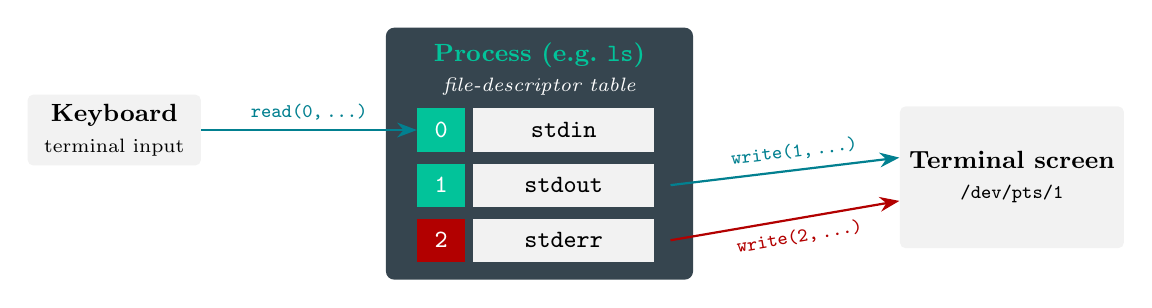
\begin{tikzpicture}[b/.style={rectangle,rounded corners=2pt,minimum height=0.9cm,align=center,font=\small},
  fd/.style={rectangle,minimum width=0.6cm,minimum height=0.55cm,font=\ttfamily\small\bfseries,text=white},
  nm/.style={rectangle,fill=light,minimum width=2.3cm,minimum height=0.55cm,font=\ttfamily\small},
  arr/.style={-{Stealth[length=2.5mm]},thick}]
\node[b,fill=light,minimum width=2.2cm] (kb) at (-0.8,-0.3) {\textbf{Keyboard}\\{\scriptsize terminal input}};
\node[rectangle,rounded corners=3pt,fill=charcoal,minimum width=3.9cm,minimum height=3.2cm] (p) at (4.6,-0.6) {};
\node[font=\small\bfseries,text=mint] at (4.6,0.65) {Process (e.g.\ \texttt{ls})};
\node[font=\scriptsize\itshape,text=white!70] at (4.6,0.25) {file-descriptor table};
\node[fd,fill=mint] (f0) at (3.35,-0.3) {0}; \node[nm,anchor=west] (n0) at (3.75,-0.3) {stdin};
\node[fd,fill=mint] (f1) at (3.35,-1.0) {1}; \node[nm,anchor=west] (n1) at (3.75,-1.0) {stdout};
\node[fd,fill=red!70!black] (f2) at (3.35,-1.7) {2}; \node[nm,anchor=west] (n2) at (3.75,-1.7) {stderr};
\node[b,fill=light,minimum width=2.6cm,minimum height=1.8cm] (scr) at (10.6,-0.9) {\textbf{Terminal screen}\\{\scriptsize\ttfamily /dev/pts/1}};
\draw[arr,mintdeep] (kb.east) -- node[above,font=\scriptsize\ttfamily]{read(0,\,\dots)} (f0.west);
\draw[arr,mintdeep] ([xshift=0.2cm]n1.east) -- node[above,font=\scriptsize\ttfamily,sloped,pos=0.55]{write(1,\,\dots)} (scr.west |- 0,-0.65);
\draw[arr,red!70!black] ([xshift=0.2cm]n2.east) -- node[below,font=\scriptsize\ttfamily,sloped,pos=0.55]{write(2,\,\dots)} (scr.west |- 0,-1.2);
\end{tikzpicture}
\caption{The three standard streams. Output and errors are two separate channels that, by default, end on the same screen.}
\label{fig:streams}
\end{figure}

Who opened them? The shell, or more precisely the chain of processes that started the shell. A child process created with \cmd{fork()} receives a copy of its parent's descriptor table, and \cmd{exec()} keeps it (Week~3). So when \cmd{bash} runs \cmd{ls}, \cmd{ls} inherits \cmd{bash}'s descriptors $0$, $1$, $2$, all pointing to the terminal.

Why two output channels? Imagine \cmd{ls} saves its listing in a file and one of its arguments does not exist. If the error message were mixed into the listing, it would end up hidden in the file. Because errors travel on their own descriptor, they still reach the screen. This simple design decision is the reason the \cmd{2>} redirection exists.

\subsection{You have seen this before: \texttt{write(1, \dots)}}

In Week~2, \cmd{strace} showed that \cmd{printf("Hello\dots")} ends up as the system call \cmd{write(1, "Hello\dots", n)}, and in Week~3 we executed the same call by hand with the \texttt{syscall} instruction: the first parameter, $1$, was standard output. Let us trace \cmd{ls} with one existing and one missing argument (\cmd{-o t1.txt} writes the trace into a file so that it does not mix with the output of \cmd{ls}):

\lstinputlisting[style=term,linerange={1-12}]{../code/out_strace.txt}

The four pieces of the error message go out with \cmd{write(2, \dots)}, the listing with \cmd{write(1, \dots)}. The program \cmd{ls} never asks \emph{where} descriptors $1$ and $2$ lead; that was decided before it started. If the shell makes descriptor $1$ point to a file, every \cmd{write(1, \dots)} lands in the file. That is all redirection is.

\paragraph{A small surprise.} On the terminal, \cmd{ls} printed \texttt{cities.txt\ \ numbers.txt\ \ students.csv} in columns, but the trace (and every file into which we redirect it, below) contains one name per line. \cmd{ls} checks with the library function \cmd{isatty(1)} whether descriptor $1$ is a terminal and chooses its format accordingly. Most programs do not care; a few (\cmd{ls}, \cmd{grep -{}-color=auto}) do.

\subsection{Seeing the descriptors: \texttt{/proc/self/fd}}

The \texttt{/proc} file system (Week~3) shows the kernel's view of every process. \texttt{/proc/self} is the process that is looking, and \texttt{/proc/self/fd} lists its descriptors as symbolic links. Running \cmd{ls -l /proc/self/fd} therefore shows the descriptors of \cmd{ls} itself:

\lstinputlisting[style=term,linerange={5-23}]{../code/out_streams.txt}

\begin{itemize}
  \item Normally, $0$, $1$ and $2$ all point to the terminal device \texttt{/dev/pts/1}. Descriptor $3$ is the directory that \cmd{ls} is reading at that moment.
  \item With \cmd{> fd.txt}, descriptor $1$ points to the file \texttt{/home/student/lab/fd.txt}; \cmd{ls} wrote its own listing into it. The mode \texttt{l-wx------} shows that the file is open for writing only.
  \item With \cmd{< docs/syllabus.txt}, descriptor $0$ is the file, opened read-only (\texttt{lr-x------}).
  \item With \cmd{2> /dev/null} (see \texttt{code/out\_streams.txt}), descriptor $2$ points to \texttt{/dev/null}.
\end{itemize}

% =====================================================================
\section{Redirection}
\label{sec:redir}

\subsection{Output: \texttt{>} and \texttt{>>}}

\lstinputlisting[style=term,linerange={1-10}]{../code/out_redirect.txt}

\cmd{cmd > file} creates the file if necessary, \emph{empties it} (truncates it to $0$ bytes) and connects descriptor $1$ to it. \cmd{cmd >> file} opens it for \emph{appending}: new data goes to the end. The third \cmd{echo} above replaced both lines: the old content is gone, with no undo and no recycle bin (Week~10). Bash can protect you: after \cmd{set -o noclobber}, the shell refuses to overwrite an existing file with \cmd{>} (the operator \cmd{>|} forces it).

\subsection{Input: \texttt{<}}

\lstinputlisting[style=term,linerange={11-14}]{../code/out_redirect.txt}

With \cmd{wc -l logs/access.log}, \cmd{wc} opens the file itself and knows its name, so it prints the name. With \cmd{wc -l < logs/access.log}, the \emph{shell} opens the file as descriptor $0$ and \cmd{wc} just reads its standard input: it has no name to print. The bare number is handy in scripts (Week~14).

\begin{keyidea}[The filter convention]
Most text tools are \term{filters}: they read the files named on the command line, or standard input if no file is named, and write their result to standard output. Error messages go to standard error. Because of this convention, any filter can be fed from a file, from the keyboard, or from another program --- and its output can go to the screen, to a file, or to another program.
\end{keyidea}

\subsection{Errors: \texttt{2>}, \texttt{2>\&1}, \texttt{\&>} and \texttt{/dev/null}}

The general form of a redirection is \texttt{n>file}, where \texttt{n} is a descriptor number; \texttt{>} alone means \texttt{1>}, and \texttt{<} alone means \texttt{0<}.

\lstinputlisting[style=term,linerange={15-33}]{../code/out_redirect.txt}
\lstinputlisting[style=term,linerange={41-44}]{../code/out_redirect.txt}

\begin{itemize}
  \item \cmd{> out.txt} moves only standard output, so the error still appears on the screen.
  \item \cmd{2> err.txt} moves only standard error: the listing appears, the error is in the file.
  \item \cmd{> all.txt 2>\&1} puts both in the file. \cmd{2>\&1} reads ``make descriptor $2$ a copy of descriptor $1$''.
  \item \cmd{\&> all.txt} is a bash shorthand for the same thing (it does not work in the simpler \cmd{sh}/\cmd{dash}).
  \item \cmd{2> /dev/null} throws the errors away. \texttt{/dev/null} is a \emph{device file}: whatever is written to it disappears, and reading from it immediately returns end-of-file.
\end{itemize}

\subsection{Order matters}

Redirections are processed \emph{from left to right}, and \cmd{2>\&1} copies descriptor $1$ \emph{as it is at that moment}; it is not a permanent link. Compare:

\lstinputlisting[style=term,linerange={34-40}]{../code/out_redirect.txt}

\begin{figure}[H]
\centering
\resizebox{\linewidth}{!}{%
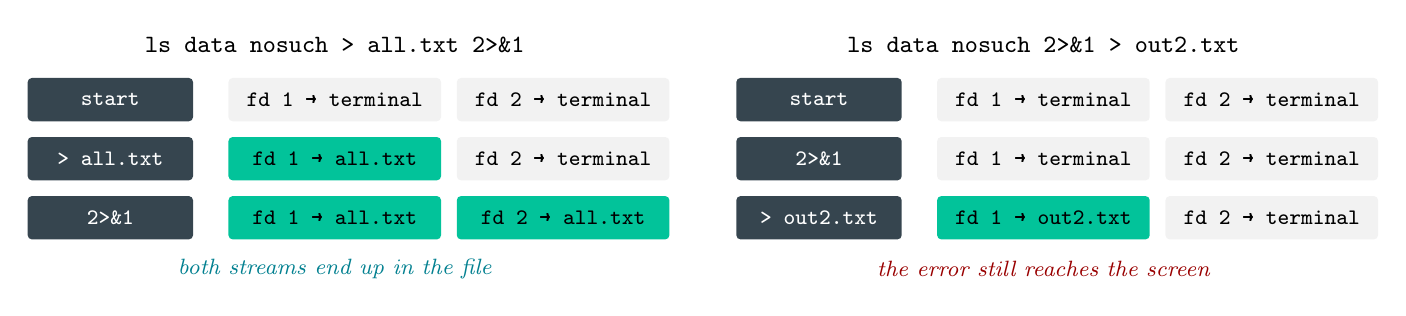
\begin{tikzpicture}[st/.style={rectangle,rounded corners=1.5pt,fill=charcoal,text=white,minimum width=2.1cm,minimum height=0.55cm,font=\ttfamily\footnotesize},
  t/.style={rectangle,rounded corners=1.5pt,fill=light,minimum width=2.7cm,minimum height=0.55cm,font=\ttfamily\footnotesize},
  f/.style={rectangle,rounded corners=1.5pt,fill=mint,minimum width=2.7cm,minimum height=0.55cm,font=\ttfamily\footnotesize\bfseries}]
\begin{scope}
\node[font=\small\ttfamily\bfseries] at (2.85,0.7) {ls data nosuch > all.txt 2>\&1};
\node[st] at (0,0) {start}; \node[t] at (2.85,0) {fd 1 → terminal}; \node[t] at (5.75,0) {fd 2 → terminal};
\node[st] at (0,-0.75) {> all.txt}; \node[f] at (2.85,-0.75) {fd 1 → all.txt}; \node[t] at (5.75,-0.75) {fd 2 → terminal};
\node[st] at (0,-1.5) {2>\&1}; \node[f] at (2.85,-1.5) {fd 1 → all.txt}; \node[f] at (5.75,-1.5) {fd 2 → all.txt};
\node[font=\footnotesize\itshape,text=mintdeep] at (2.85,-2.15) {both streams end up in the file};
\end{scope}
\begin{scope}[xshift=9.0cm]
\node[font=\small\ttfamily\bfseries] at (2.85,0.7) {ls data nosuch 2>\&1 > out2.txt};
\node[st] at (0,0) {start}; \node[t] at (2.85,0) {fd 1 → terminal}; \node[t] at (5.75,0) {fd 2 → terminal};
\node[st] at (0,-0.75) {2>\&1}; \node[t] at (2.85,-0.75) {fd 1 → terminal}; \node[t] at (5.75,-0.75) {fd 2 → terminal};
\node[st] at (0,-1.5) {> out2.txt}; \node[f] at (2.85,-1.5) {fd 1 → out2.txt}; \node[t] at (5.75,-1.5) {fd 2 → terminal};
\node[font=\footnotesize\itshape,text=red!60!black] at (2.85,-2.15) {the error still reaches the screen};
\end{scope}
\end{tikzpicture}}
\caption{The descriptor table after each redirection, processed left to right.}
\label{fig:order}
\end{figure}

\subsection{How the shell does it}
\label{sec:dup2}

In Week~3 we asked why UNIX creates processes with two separate calls, \cmd{fork()} and \cmd{exec()}, and answered: between them, the child can prepare its environment, for example redirect its output. Here is the proof. We trace a non-interactive \cmd{bash} running \cmd{ls data > list.txt}, following children (\cmd{-f}) and showing only three system calls:

\lstinputlisting[style=term,linerange={13-18}]{../code/out_strace.txt}

The first number on each line is the PID: $15726$ is \cmd{bash}, $15727$ its child (created with \cmd{clone()}, the Linux system call behind \cmd{fork()}, not traced here). The child
\begin{enumerate}[leftmargin=1.4em]
  \item opens \texttt{list.txt} for writing; \texttt{O\_CREAT} creates it, \texttt{O\_TRUNC} empties it (that is the ``\cmd{>} destroys the old content'' of the previous section), and the kernel returns the lowest free descriptor, $3$;
  \item calls \cmd{dup2(3, 1)}: descriptor $1$ becomes a copy of descriptor $3$, so standard output now leads to the file (the shell then closes the spare descriptor $3$);
  \item calls \cmd{execve("/usr/bin/ls", \dots)}: the program is replaced by \cmd{ls}, but the descriptor table survives. \cmd{ls} writes to descriptor $1$ --- the file --- and never knows it was redirected.
\end{enumerate}
In the same way, \cmd{>>} opens with \texttt{O\_APPEND} instead of \texttt{O\_TRUNC}, \cmd{<} opens read-only and duplicates onto descriptor $0$, and \cmd{2>\&1} is simply \cmd{dup2(1, 2)}. Redirection is not a feature of \cmd{ls} or of any other command: it is done by the shell, with ordinary system calls.

% =====================================================================
\section{Pipes}
\label{sec:pipes}

\subsection{Connecting processes}

Redirection connects a process to a \emph{file}. A \term{pipe}, written \cmd{cmd1 | cmd2}, connects a process to another \emph{process}: the standard output of \cmd{cmd1} becomes the standard input of \cmd{cmd2}. A chain of commands joined by pipes is a \term{pipeline}.

\begin{figure}[H]
\centering
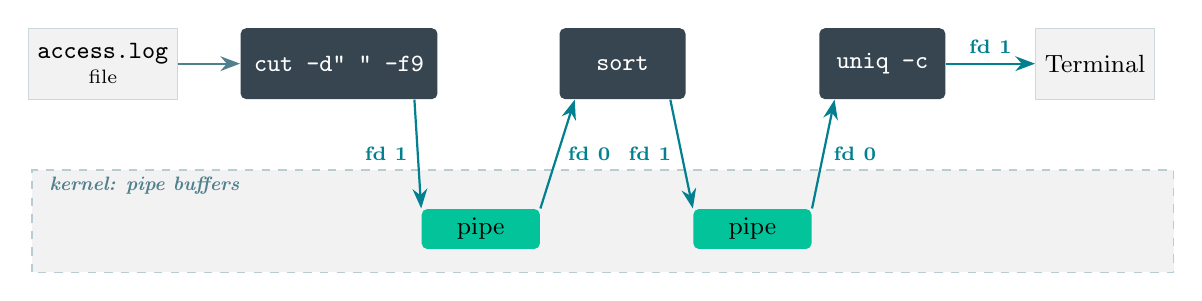
\begin{tikzpicture}[pr/.style={rectangle,rounded corners=2pt,fill=charcoal,text=white,minimum height=0.9cm,align=center,font=\ttfamily\small},
  pp/.style={rectangle,rounded corners=2pt,fill=mint,minimum width=1.5cm,minimum height=0.5cm,font=\small},
  arr/.style={-{Stealth[length=2.5mm]},thick,mintdeep}, lb/.style={font=\scriptsize\bfseries,text=mintdeep}]
\fill[light,draw=slate!40,dashed] (-0.9,-2.65) rectangle (13.6,-1.35);
\node[font=\scriptsize\itshape\bfseries,text=slate,anchor=west] at (-0.8,-1.55) {kernel: pipe buffers};
\node[rectangle,fill=light,draw=slate!30,minimum height=0.9cm,font=\ttfamily\small,align=center] (file) at (0,0) {access.log\\[-2pt]{\scriptsize\rmfamily file}};
\node[pr,minimum width=2.5cm] (cut) at (3.0,0) {cut -d" " -f9};
\node[pr,minimum width=1.6cm] (sort) at (6.6,0) {sort};
\node[pr,minimum width=1.6cm] (uniq) at (9.9,0) {uniq -c};
\node[rectangle,fill=light,draw=slate!30,minimum height=0.9cm,font=\small] (term) at (12.6,0) {Terminal};
\node[pp] (p1) at (4.8,-2.1) {pipe}; \node[pp] (p2) at (8.25,-2.1) {pipe};
\draw[arr,slate] (file) -- (cut);
\draw[arr] (cut.south east) ++(-0.3,0) -- node[lb,left]{fd 1} (p1.north west);
\draw[arr] (p1.north east) -- node[lb,right]{fd 0} ([xshift=0.2cm]sort.south west);
\draw[arr] ([xshift=-0.2cm]sort.south east) -- node[lb,left]{fd 1} (p2.north west);
\draw[arr] (p2.north east) -- node[lb,right]{fd 0} ([xshift=0.2cm]uniq.south west);
\draw[arr] (uniq) -- node[lb,above]{fd 1} (term);
\end{tikzpicture}
\caption{The pipeline \cmd{cut -d" " -f9 logs/access.log | sort | uniq -c}: three processes running at the same time, connected through two buffers inside the kernel. Standard error (fd~$2$) of every stage still goes to the terminal.}
\label{fig:pipeline}
\end{figure}

\lstinputlisting[style=term,linerange={11-17}]{../code/out_analysis.txt}

\cmd{cut} extracts field~$9$ (the HTTP status code) from each line, \cmd{sort} brings equal codes together, \cmd{uniq -c} counts each group. No temporary files are created: the data flows through memory buffers owned by the kernel. Each stage is an independent process with its own PID (Week~3), and the shell starts all of them.

\subsection{How the shell builds a pipe}

A pipe is created with the system call \cmd{pipe()} (in modern Linux \cmd{pipe2()}), which returns \emph{two} descriptors: one for reading and one for writing. Tracing a two-stage pipeline:

\lstinputlisting[style=term,linerange={19-29}]{../code/out_strace.txt}

\begin{enumerate}[leftmargin=1.4em]
  \item \cmd{pipe2([3, 4], 0)}: \cmd{bash} ($15736$) gets a pipe: descriptor $3$ is the read end, $4$ the write end.
  \item Two \cmd{clone()} calls (= \cmd{fork()}) create the children $15737$ and $15738$; both inherit descriptors $3$ and $4$.
  \item The first child calls \cmd{dup2(4, 1)}: its standard output is now the write end. It then executes \cmd{grep}.
  \item The second child calls \cmd{dup2(3, 0)}: its standard input is the read end. It executes \cmd{wc}.
  \item Unused ends are closed (\cmd{close()} was not traced), and \cmd{bash} waits for both children (the remaining lines of the trace, omitted here, show the two exits and the \texttt{SIGCHLD} signal with which the kernel tells the parent that a child has terminated).
\end{enumerate}
Notice that \cmd{wc} was executed \emph{before} \cmd{grep} in this run: the two children run concurrently, and the scheduler (Week~4) decides who goes first. When two processes make system calls at the same moment, \cmd{strace} may print a call in two halves, marked \texttt{<unfinished \dots>} and \texttt{<\dots{} resumed>}; that is normal.

A pipe is visible in \texttt{/proc} too: in \cmd{ls -l /proc/self/fd | cat}, the descriptor $1$ of \cmd{ls} is shown as \texttt{1 -> pipe:[29942]}, a pipe identified by a number inside the kernel (full output in \texttt{code/out\_pipes.txt}).

\begin{keyidea}[Redirection and pipes in four system calls]
\cmd{pipe()} creates the channel, \cmd{fork()} creates the processes, \cmd{dup2()} plugs the channel (or a file opened with \cmd{open()}) into descriptor $0$, $1$ or $2$, and \cmd{exec()} starts the program, which inherits the plumbing without knowing it.
\end{keyidea}

\subsection{A pipe is a bounded buffer (Week 5)}

A pipe has a limited capacity: on Linux the default is $64$~KiB $= 16 \times 4096 = 65\,536$ bytes (sixteen $4$~KiB pages). The kernel enforces three rules:
\begin{itemize}
  \item \textbf{Buffer full:} \cmd{write()} blocks --- the writer is put to sleep until the reader has removed data.
  \item \textbf{Buffer empty:} \cmd{read()} blocks --- the reader sleeps until data arrives.
  \item \textbf{No writer left and buffer empty:} \cmd{read()} returns $0$, which means end-of-file; the reader finishes. \textbf{No reader left:} the writer receives the signal \texttt{SIGPIPE}, which terminates it.
\end{itemize}
This is exactly the \emph{bounded-buffer} (producer--consumer) problem of Week~5, solved inside the kernel: the producer must wait when the buffer is full, the consumer when it is empty. Two experiments show the consequences:

\lstinputlisting[style=term,linerange={9-19}]{../code/out_pipes.txt}

\cmd{sleep 2 | sleep 2} takes $2.0$~s, not $4$~s: the stages run \emph{concurrently}. \cmd{yes} prints \texttt{y} forever, yet the pipeline stops: after three lines \cmd{head} exits, the pipe has no reader, and the next \cmd{write()} of \cmd{yes} triggers \texttt{SIGPIPE}. (Signals are a topic of Week~13.) The last pipeline pushes $100\,000$ lines, about $800$~kB, through two $64$~KiB buffers without any problem: data is consumed as fast as it is produced.

\begin{histnote}[Pipes and the UNIX philosophy]
In a 1964 memo, Doug McIlroy at Bell Labs wrote that programs should be connected ``like garden hose --- screw in another segment when it becomes necessary to massage data in another way''. Pipes appeared in UNIX Version~3 in 1973, when Ken Thompson added the \cmd{pipe()} system call and the \texttt{|} notation to the shell. McIlroy later summarised the resulting style: write programs that do one thing and do it well; write programs to work together; write programs to handle text streams, because that is a universal interface. \cmd{grep} itself is named after the command \texttt{g/re/p} (``global regular expression print'') of the \cmd{ed} text editor.
\end{histnote}

% =====================================================================
\section{Searching Lines: \texttt{grep}}
\label{sec:grep}

\cmd{grep [options] PATTERN [files]} prints the lines that contain the pattern.

\lstinputlisting[style=term,linerange={1-20}]{../code/out_grep.txt}

\begin{center}
\renewcommand{\arraystretch}{1.2}
\begin{tabular}{@{}lp{11.5cm}@{}}
\toprule
\textbf{Option} & \textbf{Meaning}\\
\midrule
\cmd{-i} & ignore the difference between upper and lower case\\
\cmd{-n} & prefix each line with its line number\\
\cmd{-v} & invert: print the lines that do \emph{not} match\\
\cmd{-c} & print only the number of matching \emph{lines} (not occurrences)\\
\cmd{-w} & the match must be a whole word\\
\cmd{-r} & search all files below a directory (recursively)\\
\cmd{-l} & print only the names of files that contain a match\\
\bottomrule
\end{tabular}
\end{center}

Options can be combined: \cmd{grep -vc INFO} counts the non-INFO lines, $41$. (Later we will see that these are $13$ ERROR and $28$ WARN lines, and $13 + 28 = 41$.) The minutes in \texttt{system.log} are not in order within an hour; this is generated practice data, while real logs are in time order.

\subsection{Whole words and whole directories}

\lstinputlisting[style=term,linerange={21-33}]{../code/out_grep.txt}

The pattern \texttt{Week 1} also occurs inside \texttt{Week 10} \dots\ \texttt{Week 15}. With \cmd{-w}, the match must not be preceded or followed by a letter, digit or underscore. With \cmd{-r}, \cmd{grep} searches every file below \texttt{projects} and prefixes each line with the file name; the files appear in directory order, not alphabetically.

\subsection{Simple regular expressions}

The pattern of \cmd{grep} is a \term{regular expression} (regex): a small language for describing sets of strings. Most characters match themselves; a few have a special meaning.

\begin{center}
\renewcommand{\arraystretch}{1.2}
\begin{tabular}{@{}lp{4.6cm}lp{3.6cm}@{}}
\toprule
\textbf{Symbol} & \textbf{Matches} & \textbf{Example} & \textbf{Matches, e.g.}\\
\midrule
\texttt{\textasciicircum} & the start of the line & \texttt{\textasciicircum Week} & lines beginning with \texttt{Week}\\
\texttt{\$} & the end of the line & \texttt{s\$} & lines ending in \texttt{s}\\
\texttt{.} & any \emph{one} character & \texttt{c.de} & \texttt{code}, \texttt{cxde}\\
\texttt{[ ]} & one character from a set or range & \texttt{[0-9]}, \texttt{[aeiou]} & \texttt{7}, \texttt{e}\\
\texttt{*} & the preceding item, $0$ or more times & \texttt{[0-9]*} & empty, \texttt{4}, \texttt{2026}\\
\texttt{\textbackslash.} & a literal dot (\texttt{\textbackslash} removes the special meaning) & \texttt{5\textbackslash.38} & \texttt{5.38} only\\
\bottomrule
\end{tabular}
\end{center}

\begin{lstlisting}[style=term]
student@okan-lab:~/lab$ grep "^Week [0-9] " docs/syllabus.txt
Week 1  Introduction and history
Week 2  Definitions, goals, components, structures
Week 3  OS services, system calls, processes
...
student@okan-lab:~/lab$ grep "s$" docs/syllabus.txt
Week 2  Definitions, goals, components, structures
Week 3  OS services, system calls, processes
Week 4  Threads and CPU scheduling basics
...
student@okan-lab:~/lab$ grep "c.de" docs/linux_quotes.txt
Talk is cheap. Show me the code.
student@okan-lab:~/lab$ grep -c "5.38" logs/access.log
39
student@okan-lab:~/lab$ grep -c "5\.38" logs/access.log
37
student@okan-lab:~/lab$ grep "5.38" logs/access.log | grep -v "5\.38"
10.0.6.45 - - [12/Oct/2026:15:53:47 +0300] "GET /courses/mcmp117 HTTP/1.1" 200 5438
10.0.2.17 - - [12/Oct/2026:15:38:02 +0300] "GET /login HTTP/1.1" 200 1357
student@okan-lab:~/lab$ grep ",ECT,[0-9]*,9[0-9]$" data/students.csv
2026001,Elif Yilmaz,ECT,96,99
2026015,Deniz Celik,ECT,95,96
student@okan-lab:~/lab$ grep "^2026-10-12 1[0-1]:.*ERROR" logs/system.log
2026-10-12 10:40:00 ERROR failed to mount /dev/sdb1
2026-10-12 10:35:00 ERROR failed to mount /dev/sdb1
2026-10-12 10:30:00 ERROR failed to mount /dev/sdb1
2026-10-12 10:03:00 ERROR failed to mount /dev/sdb1
\end{lstlisting}

\begin{itemize}
  \item \texttt{\textasciicircum Week [0-9] } (note the final space) matches \texttt{Week}, a space, one digit and a space at the start of the line: the single-digit weeks $1$--$9$.
  \item The unescaped dot is a classic trap. Counting the requests of the IP address \texttt{10.0.5.38} with the pattern \texttt{5.38} gives $39$, but the correct answer is $37$: the dot also matched the \texttt{:} in the time \texttt{15:38} and the digit \texttt{4} in the byte count \texttt{5438}. The last \cmd{grep} pipeline shows exactly those two extra lines.
  \item \texttt{,ECT,[0-9]*,9[0-9]\$} finds ECT students whose \emph{final} grade (the last field) is between $90$ and $99$.
  \item \texttt{.*} means ``any number of any characters'': \texttt{\textasciicircum 2026-10-12 1[0-1]:.*ERROR} finds ERROR lines between $10$:00 and $11$:59.
\end{itemize}

\begin{keyidea}[Regular expressions are not wildcards]
In the shell (Week~10), \texttt{*} means ``any string'' and \texttt{?} ``any character''. In a regular expression, \texttt{*} means ``repeat the previous item'' and \texttt{.} means ``any character''. Always put the pattern in quotes, so that the shell does not try to expand \texttt{*}, \texttt{[ ]} or spaces before \cmd{grep} sees them. (\cmd{grep -E} enables \emph{extended} regular expressions with \texttt{+}, \texttt{?}, \texttt{|} and groups; we do not need them this week.)
\end{keyidea}

% =====================================================================
\section{Sorting and Counting: \texttt{sort} and \texttt{uniq}}
\label{sec:sort}

\lstinputlisting[style=term,linerange={1-17}]{../code/out_sort_uniq.txt}

Without options, \cmd{sort} compares lines \emph{character by character}, so \texttt{100} comes before \texttt{35} (the character \texttt{1} is smaller than \texttt{3}). With \cmd{-n} it compares numbers. Main options:

\begin{center}
\renewcommand{\arraystretch}{1.2}
\begin{tabular}{@{}lp{11.5cm}@{}}
\toprule
\cmd{-n} & numeric order ($35 < 100$)\\
\cmd{-r} & reverse order (largest first)\\
\cmd{-t,} & the field separator is a comma (default: blanks)\\
\cmd{-k5} & sort by field $5$ (from field $5$ to the end of the line; \cmd{-k5,5} means field $5$ only)\\
\cmd{-u} & output each distinct line only once\\
\cmd{-o file} & write the result to \emph{file}; safe even if \emph{file} is the input\\
\bottomrule
\end{tabular}
\end{center}

The command \cmd{tail -n +2} prints a file from line~$2$ onwards, skipping the CSV header \texttt{id,\allowbreak name,\allowbreak department,\allowbreak midterm,\allowbreak final}; see Section~\ref{sec:errors} for what happens if you forget it.

\cmd{uniq} removes \emph{adjacent} duplicate lines; \cmd{-c} prefixes each line with the number of repeats, \cmd{-d} prints only lines that are repeated. Because \cmd{uniq} compares a line only with the line just before it, it must almost always follow \cmd{sort}:

\lstinputlisting[style=term,linerange={18-40}]{../code/out_sort_uniq.txt}

On the unsorted file \cmd{uniq -c} reports \texttt{1 Antalya}, although Antalya occurs $6$ times: the six lines are not next to each other. After \cmd{sort} the counts are right, and they add up: $2 + 6 + 5 + 5 + 1 + 2 + 4 + 5 = 30$ lines. The combination
\[
\texttt{sort | uniq -c | sort -rn}
\]
answers ``how many of each, most frequent first'' and is the most useful pipeline of this week. Equal counts (Trabzon and Eskisehir, $5$ each) are ordered by the rest of the line, reversed by \cmd{-r}. Finally, \cmd{uniq -d} shows that four names occur twice in \texttt{students.csv}: different students (different ids) who happen to share a name.

% =====================================================================
\section{Columns, Counts and Characters: \texttt{cut}, \texttt{wc}, \texttt{tr}}
\label{sec:cut}

\subsection{\texttt{cut}}

\lstinputlisting[style=term,linerange={1-23}]{../code/out_cut_tr_wc.txt}

\cmd{cut -d SEP -f LIST} splits each line at the single character \texttt{SEP} and keeps the listed fields (counted from $1$): \cmd{-f2,5} fields $2$ and $5$, \cmd{-f2-4} fields $2$ to $4$, \cmd{-f4-} field $4$ to the end. \cmd{cut -c 12-16} keeps characters $12$ to $16$, useful for fixed-width columns.

In \texttt{system.log} the level is padded to five characters (\texttt{INFO\textvisiblespace\textvisiblespace network}), so between \texttt{INFO} and the message there are \emph{two} spaces. \cmd{cut} treats each space as a separator, sees an empty field between them, and field~$4$ is empty --- hence the three empty lines. \cmd{tr -s " "} squeezes runs of spaces into one space first.

\subsection{\texttt{wc}}

\lstinputlisting[style=term,linerange={24-30}]{../code/out_cut_tr_wc.txt}

\cmd{wc} prints the number of lines, words and bytes: \texttt{system.log} has $120$ lines, $669$ words and $5207$ bytes. \cmd{-l}, \cmd{-w} and \cmd{-c} select one count; with several files a \texttt{total} line is added. The line count is the number of newline characters, so a last line without a newline is not counted.

\subsection{\texttt{tr}}

\lstinputlisting[style=term,linerange={31-38}]{../code/out_cut_tr_wc.txt}

\cmd{tr SET1 SET2} replaces every character of \texttt{SET1} by the corresponding character of \texttt{SET2}; \cmd{tr -d SET} deletes characters; \cmd{tr -s SET} squeezes repeats. \cmd{tr} works on single characters, not words (\cmd{tr "cat" "dog"} replaces c by d, a by o and t by g everywhere), and it reads only standard input: it never takes a file name, so use \cmd{<} or a pipe.

% =====================================================================
\section{More Tools: \texttt{head}, \texttt{tail}, \texttt{tee}, \texttt{find}, \texttt{xargs}}
\label{sec:more}

\subsection{\texttt{head} and \texttt{tail} in pipelines; \texttt{tee}}

\lstinputlisting[style=term,linerange={7-18}]{../code/out_head_tail_tee.txt}

\cmd{head -n N} keeps the first $N$ lines, \cmd{tail -n N} the last $N$, and \cmd{tail -n +N} everything from line $N$ on. Combined, \cmd{head -n 120 | tail -n 1} extracts exactly line $120$. \cmd{tail -f file} keeps the file open and prints new lines as they are appended: the standard way to watch a log live (stop with Ctrl+C).

\cmd{tee file} is a T-junction (named after the plumber's T-piece): it copies its standard input both to the file and to its standard output, so a pipeline can save an intermediate result and continue. \cmd{tee -a} appends. A link to Week~11: \cmd{sudo echo text > /etc/file} fails, because the redirection is performed by \emph{your} shell, without root rights, before \cmd{sudo} even starts; \cmd{echo text | sudo tee /etc/file} works because the file is opened by \cmd{tee}, which runs as root.

\subsection{\texttt{find}}

\cmd{find WHERE TESTS} walks the whole directory tree below \texttt{WHERE} and prints every path that passes all tests.

\lstinputlisting[style=term,linerange={1-18}]{../code/out_find_xargs.txt}

\begin{center}
\renewcommand{\arraystretch}{1.2}
\begin{tabular}{@{}lp{10.5cm}@{}}
\toprule
\textbf{Test} & \textbf{Meaning}\\
\midrule
\cmd{-name "*.txt"} & the name matches the wildcard pattern (keep the quotes!)\\
\cmd{-iname} & the same, ignoring case\\
\cmd{-type f}, \cmd{-type d} & regular file, directory\\
\cmd{-size +10k}, \cmd{-size -10k} & larger / smaller than $10$~KiB $= 10\,240$ bytes\\
\cmd{-mtime +30}, \cmd{-mtime -1} & modified more than $30$ days ago / within the last $24$ hours\\
\bottomrule
\end{tabular}
\end{center}

Without the quotes in \cmd{-name "*.txt"}, the shell would expand \texttt{*.txt} in the \emph{current} directory before \cmd{find} starts (Week~10). Only \texttt{access.log} ($23\,604$ bytes) exceeds $10$~KiB. The $14$ photos are the twelve \texttt{img0NN.jpg}, \texttt{IMG\_014.JPG} and \texttt{holiday.jpeg}; \texttt{img013.png} does not match. Since all lab files were just created, we used \cmd{touch -d} to give \texttt{notes\_01.txt} an old modification time (Week~10) so that \cmd{-mtime +30} finds something. Like \cmd{grep -r}, \cmd{find} lists entries in directory order; pipe into \cmd{sort} if you need a fixed order.

\paragraph{Errors from \texttt{find}.} When \cmd{find} meets a directory it may not read (Week~11), it reports an error --- on standard error, so it can be discarded separately:
\lstinputlisting[style=term,linerange={45-52}]{../code/out_find_xargs.txt}
(We removed the permissions of \texttt{secret} with \cmd{chmod 000}; afterwards, restore them with \cmd{chmod 755 secret} and remove it with \cmd{rmdir secret}.)

\subsection{\texttt{-exec} and \texttt{xargs}}

\lstinputlisting[style=term,linerange={19-44}]{../code/out_find_xargs.txt}

\begin{itemize}
  \item \cmd{-exec cmd \{\} \textbackslash;} runs \cmd{cmd} once for every file found, with \texttt{\{\}} replaced by its name. The \texttt{\textbackslash;} marks the end of the command (the backslash stops the shell from interpreting \texttt{;}).
  \item \cmd{xargs cmd} reads words from its standard input and passes them to \cmd{cmd} as \emph{arguments}: one \cmd{wc} receives all three names and prints a total. This is the difference between data and arguments: \cmd{find \dots{} | wc -l} would count the \emph{names}; \cmd{find \dots{} | xargs wc -l} counts the lines \emph{in the files}.
  \item By default \cmd{xargs} splits at spaces, so \texttt{final report.txt} became two non-existent names, \texttt{docs/\allowbreak final} and \texttt{report.txt}, and the total ($23$) missed its $2$ lines. \cmd{find -print0} ends each name with a zero byte (which cannot occur in a file name) and \cmd{xargs -0} splits only there: total $25$.
\end{itemize}

\begin{tryit}[Safety: look before you delete]
\cmd{find \dots{} -exec rm \{\} \textbackslash;} and \cmd{find \dots{} | xargs rm} delete every file in the list, without asking and without a recycle bin. Always run the same command \emph{without} \cmd{rm} first, read the list, and only then add \cmd{rm}. The same applies to \cmd{rm -r}.
\end{tryit}

% =====================================================================
\section{Real Analyses with One-Line Pipelines}
\label{sec:analysis}

\subsection{Know your data}

Before writing a pipeline, look at a few lines (\cmd{head -n 3}) and decide how the fields are separated.

\begin{figure}[H]
\centering
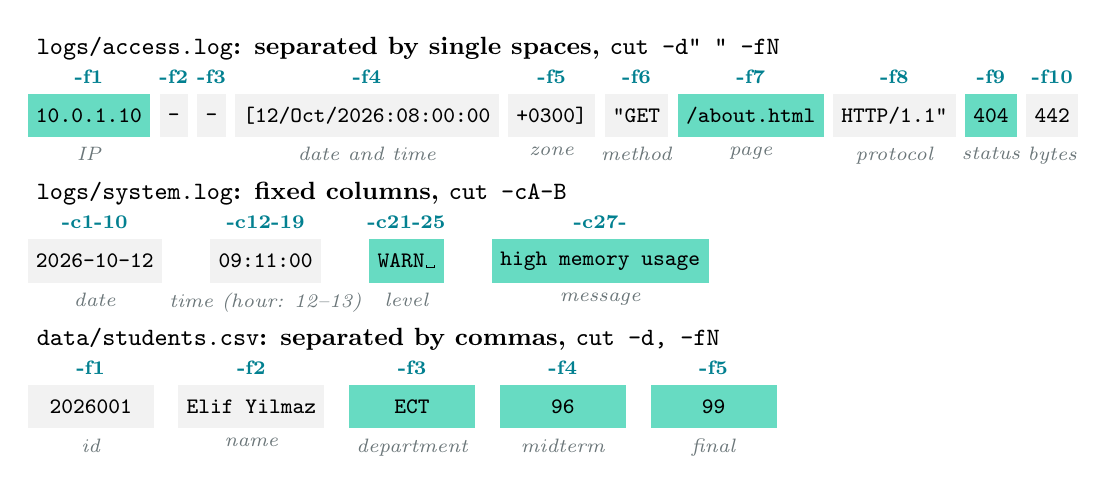
\begin{tikzpicture}[f/.style={rectangle,fill=light,minimum height=0.55cm,font=\ttfamily\footnotesize,inner xsep=3pt},
  h/.style={f,fill=mint!60}, n/.style={font=\scriptsize\bfseries,text=mintdeep}, l/.style={font=\scriptsize\itshape,text=muted}]
\node[font=\small\bfseries,anchor=west] at (0,0.85) {\texttt{logs/access.log}: separated by single spaces, \texttt{cut -d" " -fN}};
\foreach \t/\c/\lab [count=\i] in {10.0.1.10/h/IP, -/f/{}, -/f/{}, {[12/Oct/2026:08:00:00}/f/date and time, +0300]/f/zone, "GET/f/method, {/about.html}/h/page, {HTTP/1.1"}/f/protocol, 404/h/status, 442/f/bytes} {
  \ifnum\i=1 \node[\c,anchor=west] (a\i) at (0,0) {\t};
  \else \pgfmathtruncatemacro{\j}{\i-1}\node[\c,anchor=west] (a\i) at ([xshift=3pt]a\j.east) {\t}; \fi
  \node[n,above=0pt of a\i] {-f\i};
  \node[l,below=0pt of a\i] {\lab};
}
\node[font=\small\bfseries,anchor=west] at (0,-1.0) {\texttt{logs/system.log}: fixed columns, \texttt{cut -cA-B}};
\node[f,anchor=west] (s1) at (0,-1.85) {2026-10-12}; \node[n,above=0pt of s1] {-c1-10}; \node[l,below=0pt of s1] {date};
\node[f,anchor=west] (s2) at ([xshift=0.6cm]s1.east) {09:11:00}; \node[n,above=0pt of s2] {-c12-19}; \node[l,below=0pt of s2] {time (hour: 12--13)};
\node[h,anchor=west] (s3) at ([xshift=0.6cm]s2.east) {WARN\textvisiblespace}; \node[n,above=0pt of s3] {-c21-25}; \node[l,below=0pt of s3] {level};
\node[h,anchor=west] (s4) at ([xshift=0.6cm]s3.east) {high memory usage}; \node[n,above=0pt of s4] {-c27-}; \node[l,below=0pt of s4] {message};
\node[font=\small\bfseries,anchor=west] at (0,-2.85) {\texttt{data/students.csv}: separated by commas, \texttt{cut -d, -fN}};
\foreach \t/\c/\lab [count=\i] in {2026001/f/id, Elif Yilmaz/f/name, ECT/h/department, 96/h/midterm, 99/h/final} {
  \ifnum\i=1 \node[\c,anchor=west,minimum width=1.6cm] (c\i) at (0,-3.7) {\t};
  \else \pgfmathtruncatemacro{\j}{\i-1}\node[\c,anchor=west,minimum width=1.6cm] (c\i) at ([xshift=0.3cm]c\j.east) {\t}; \fi
  \node[n,above=0pt of c\i] {-f\i};
  \node[l,below=0pt of c\i] {\lab};
}
\end{tikzpicture}
\caption{Where the fields are in the three lab files. Line~1 of \texttt{students.csv} is a header.}
\label{fig:fields}
\end{figure}

The web-server log uses the widespread \emph{common log format}. Field~$4$ contains date and time; to get the hour you can also cut at colons: \cmd{cut -d: -f2} gives \texttt{08}. HTTP status codes form five classes: \texttt{2xx} success (\texttt{200} OK), \texttt{3xx} redirection (\texttt{301} moved permanently, \texttt{304} not modified: use your cached copy), \texttt{4xx} client errors (\texttt{403} forbidden, \texttt{404} not found) and \texttt{5xx} server errors (\texttt{500} internal server error).

\subsection{The method: one stage at a time}

\lstinputlisting[style=term,linerange={3-10}]{../code/out_analysis.txt}
\lstinputlisting[style=term,linerange={18-24}]{../code/out_analysis.txt}

Every counting question follows the same four steps:
\begin{enumerate}[leftmargin=1.4em]
  \item \textbf{Extract} the column you need (\cmd{cut}), possibly after \textbf{filtering} the relevant lines (\cmd{grep}); check with \cmd{head}.
  \item \textbf{Group}: \cmd{sort} brings equal values together.
  \item \textbf{Count}: \cmd{uniq -c}.
  \item \textbf{Rank}: \cmd{sort -rn}, then \cmd{head -n N} for a top~$N$.
\end{enumerate}
Never type a six-stage pipeline in one go: press the up-arrow, add one stage, look at the result, repeat. Check results whenever you can. Here the counts add up to the number of lines: $148 + 57 + 34 + 24 + 20 + 17 = 300$, and the share of successful requests is $148/300 \approx 49.3\%$.

\subsection{access.log: pages, visitors, broken links}

\lstinputlisting[style=term,linerange={25-38}]{../code/out_analysis.txt}

The same recipe with field $7$ (page) and field $1$ (IP address). The third pipeline first filters the \texttt{404} lines and then extracts the page: the most frequent broken link is \texttt{/images/logo.png} ($9$ times). The spaces in \texttt{" 404 "} matter: without them, a byte count such as \texttt{4042} or an IP part could also match. Ties are common in small data: \texttt{/index.html} and \texttt{/images/logo.png} both have $33$ requests.

\subsection{system.log and students.csv}

\lstinputlisting[style=term,linerange={39-62}]{../code/out_analysis.txt}

\begin{itemize}
  \item \textbf{Errors per hour.} Here \cmd{uniq -c} works without \cmd{sort}, because the log is already in hour order, so equal hours are adjacent. Hours without errors ($11$ and $15$) are simply missing: \cmd{uniq} cannot count what is not there. Check: $3 + 4 + 1 + 3 + 2 = 13$.
  \item \textbf{Warnings.} \cmd{cut -c27-} keeps the message; $11 + 17 = 28$ WARN lines.
  \item \textbf{Departments.} $17 + 11 + 10 + 2 = 40$ students $= 41$ lines minus the header.
  \item \textbf{Best final grades.} Sort whole lines by field $5$ first, cut the display columns last; cutting first would lose the column you sort by.
\end{itemize}

% =====================================================================
\section{Command Reference}
\label{sec:ref}

{\footnotesize
\renewcommand{\arraystretch}{1.2}
\begin{longtable}{@{}p{4.6cm}p{10.9cm}@{}}
\toprule
\textbf{Command / syntax} & \textbf{Meaning}\\
\midrule
\endhead
\cmd{cmd > f} & standard output to \texttt{f} (create or empty first)\\
\cmd{cmd >> f} & standard output appended to \texttt{f}\\
\cmd{cmd < f} & standard input from \texttt{f}\\
\cmd{cmd 2> f}, \cmd{2>> f} & standard error to \texttt{f} (overwrite, append)\\
\cmd{cmd > f 2>\&1}, \cmd{cmd \&> f} & both streams to \texttt{f}\\
\cmd{cmd 2> /dev/null} & discard error messages\\
\cmd{cmd1 | cmd2} & standard output of \texttt{cmd1} to standard input of \texttt{cmd2}\\
\cmd{set -o noclobber} & \cmd{>} refuses to overwrite existing files (\cmd{>|} forces)\\
\midrule
\cmd{grep PAT files} & lines containing the regular expression \texttt{PAT}\\
\quad \cmd{-i -n -v -c -w -r -l} & ignore case, line numbers, invert, count, whole word, recursive, file names only\\
\cmd{sort} & sort lines; \cmd{-n} numeric, \cmd{-r} reverse, \cmd{-t,} separator, \cmd{-k5} key field, \cmd{-u} unique, \cmd{-o f} output file\\
\cmd{uniq} & collapse adjacent repeats; \cmd{-c} count, \cmd{-d} only repeated\\
\cmd{cut -d, -f2,5} & fields $2$ and $5$ of comma-separated lines; \cmd{-f4-} field $4$ to the end\\
\cmd{cut -c12-16} & characters $12$ to $16$\\
\cmd{wc} & lines, words, bytes; \cmd{-l}, \cmd{-w}, \cmd{-c}\\
\cmd{tr a-z A-Z} & translate characters (reads stdin only); \cmd{-d} delete, \cmd{-s} squeeze\\
\cmd{head -n N}, \cmd{tail -n N} & first / last $N$ lines\\
\cmd{tail -n +N} & from line $N$ to the end (skip a header with $N = 2$)\\
\cmd{tail -f f} & follow a growing file (Ctrl+C stops)\\
\cmd{tee f}, \cmd{tee -a f} & copy stdin to \texttt{f} and to stdout\\
\midrule
\cmd{find DIR -name "*.c"} & files below \texttt{DIR} whose name matches; \cmd{-iname} ignores case\\
\quad \cmd{-type f|d}, \cmd{-size +10k}, \cmd{-mtime +30} & file type, size, age in days\\
\quad \cmd{-exec cmd \{\} \textbackslash;} & run \texttt{cmd} on each file found\\
\quad \cmd{-print0 | xargs -0 cmd} & pass names (even with spaces) as arguments to \texttt{cmd}\\
\cmd{strace -f -e trace=\dots{} cmd} & show the system calls of \texttt{cmd} and its children\\
\bottomrule
\end{longtable}
}

% =====================================================================
\section{Common Errors and What They Mean}
\label{sec:errors}

All of the following were produced on purpose (\cmd{code/demo\_mistakes.sh}; the $15$ lines printed by the unquoted \cmd{grep} are shortened):

\begin{lstlisting}[style=term]
student@okan-lab:~/lab$ cp data/cities.txt c.txt
student@okan-lab:~/lab$ sort c.txt > c.txt
student@okan-lab:~/lab$ wc -l c.txt
0 c.txt
student@okan-lab:~/lab$ grep user login logs/system.log
grep: login: No such file or directory
logs/system.log:2026-10-12 09:44:00 INFO  user login
...
logs/system.log:2026-10-12 14:43:00 INFO  user login
logs/system.log:2026-10-12 14:27:00 INFO  user login
student@okan-lab:~/lab$ grep "user login" logs/system.log | wc -l
15
student@okan-lab:~/lab$ ls data > wc
student@okan-lab:~/lab$ ls
README.txt  c.txt  docs  photos    scripts  wc
backup      data   logs  projects  src
student@okan-lab:~/lab$ cat wc
cities.txt
numbers.txt
students.csv
student@okan-lab:~/lab$ sort -t, -k5 -n data/students.csv | head -n 2
id,name,department,midterm,final
2026032,Onur Dogan,ECT,41,35
\end{lstlisting}

\begin{description}[leftmargin=0pt,itemsep=0.3em]
  \item[\texttt{sort c.txt > c.txt} leaves an empty file.] The shell performs the redirection \emph{first}: it truncates \texttt{c.txt} to $0$ bytes, then starts \cmd{sort}, which reads an empty file. The same happens with any \cmd{cmd f > f}. Write to a new file and rename it (\cmd{sort c.txt > c2.txt \&\& mv c2.txt c.txt}), or use \cmd{sort -o c.txt c.txt}.
  \item[\texttt{grep: login: No such file or directory}.] Without quotes, the command \cmd{grep user login} \cmd{logs/system.log} searches for \texttt{user} in two files, \texttt{login} and \texttt{logs/system.log}. Quote patterns that contain spaces: \cmd{grep "user login" logs/system.log}.
  \item[A file called \texttt{wc} appears.] \cmd{ls data > wc} redirects into a file named \texttt{wc}; it does not run \cmd{wc}. Use the pipe: \cmd{ls data | wc -l}.
  \item[The header line appears in the result.] \texttt{id,name,\dots} is not a number, so \cmd{sort -n} treats it as $0$ and places it first. Skip it with \cmd{tail -n +2}.
  \item[\texttt{uniq -c} gives counts of $1$.] The input was not sorted; use \cmd{sort | uniq -c}.
  \item[Errors still appear although you wrote \texttt{2>\&1}.] The order was \cmd{2>\&1 > f}; write \cmd{> f 2>\&1} (Figure~\ref{fig:order}).
  \item[\texttt{cut} prints empty lines.] The separator occurs twice in a row (padded columns); squeeze first with \cmd{tr -s " "} or use \cmd{cut -c}.
  \item[\texttt{xargs}: \texttt{No such file or directory} for half a name.] A file name contains a space; use \cmd{find \dots{} -print0 | xargs -0 \dots}.
  \item[\texttt{Permission denied} lines from \texttt{find}.] Directories you may not read (Week~11). If they do not matter, add \cmd{2> /dev/null}.
  \item[A pipeline seems to hang.] A command without a file argument waits for input from the keyboard (e.g.\ \cmd{sort} alone, or \cmd{grep ERROR} without a file). Press Ctrl+D (end of input) or Ctrl+C.
  \item[\texttt{tr: extra operand}.] \cmd{tr} does not take file names; use \cmd{tr a-z A-Z < file}.
\end{description}

% =====================================================================
\section{Lab Sheet}
\label{sec:lab}

\textbf{Preparation:} \cmd{bash mcmp117\_lab\_setup.sh} then \cmd{cd \textasciitilde/lab}. Write one command line per exercise (a pipeline counts as one line) and its output. Points in brackets, $100$ in total. Solutions are in Section~\ref{sec:sol}; try first!

\subsection*{Part A --- Redirection (20 points)}
\begin{enumerate}[leftmargin=2.2em,label=\textbf{A\arabic*}]
  \item {[4]} Save the list of files in \texttt{data/} into \texttt{list.txt}, then append the list of \texttt{docs/} to the same file. How many lines does \texttt{list.txt} have?
  \item {[4]} Run \cmd{ls data nosuch} so that the listing goes to \texttt{ok.txt}, the error message to \texttt{err.txt}, and nothing appears on the screen.
  \item {[4]} Print only the number of lines of \texttt{logs/system.log}, without the file name.
  \item {[4]} Predict, then check: which of \cmd{ls data nosuch > both.txt 2>\&1} and \cmd{ls data nosuch 2>\&1 > both.txt} prints something on the screen, and why?
  \item {[4]} Create an unreadable directory with \cmd{mkdir secret \&\& chmod 000 secret}. The command \cmd{find . -name "*.md"} now prints an error. Change it so that only the results appear.
\end{enumerate}

\subsection*{Part B --- grep (22 points)}
\begin{enumerate}[leftmargin=2.2em,label=\textbf{B\arabic*}]
  \item {[4]} How many ERROR lines does \texttt{logs/system.log} contain?
  \item {[4]} Show the first $3$ lines of \texttt{system.log} that are \emph{not} INFO lines, with their line numbers.
  \item {[4]} How many requests in \texttt{access.log} received the status code $404$?
  \item {[4]} Which students belong to the EE department?
  \item {[6]} How many requests came from the IP address \texttt{10.0.5.38}? Make sure the dots cannot match other characters and that only the first field can match.
\end{enumerate}

\subsection*{Part C --- One-line pipelines (36 points, 6 each)}
\begin{enumerate}[leftmargin=2.2em,label=\textbf{C\arabic*}]
  \item How many students are there in each department (without the header)?
  \item Print the names and final grades of the $3$ students with the highest final grade.
  \item Count the requests per status code, most frequent first.
  \item Which are the $3$ most requested pages?
  \item Which page produced the most $404$ errors, and how many?
  \item How many ERROR lines does \texttt{system.log} contain in each hour?
\end{enumerate}

\subsection*{Part D --- Challenge (22 points)}
\begin{enumerate}[leftmargin=2.2em,label=\textbf{D\arabic*}]
  \item {[5]} Which student names appear more than once in \texttt{students.csv}?
  \item {[5]} In one command line, save all lines with status $500$ into \texttt{errors\_500.txt} \emph{and} print how many there are.
  \item {[6]} Count the lines of all \texttt{.txt} files below \texttt{docs/}, including \texttt{final report.txt}, with \cmd{find} and \cmd{xargs}. What is the total?
  \item {[6]} How many different IP addresses appear in \texttt{access.log}? Which address made the fewest requests, and how many?
\end{enumerate}

% =====================================================================
\section{Summary}

\begin{keyidea}[Week 12 in seven sentences]
\begin{enumerate}[leftmargin=1.4em]
  \item Every process starts with three open file descriptors: $0$ stdin, $1$ stdout, $2$ stderr --- the same descriptor $1$ that \cmd{write(1, \dots)} used in Weeks~2--3.
  \item Redirection (\cmd{> >> < 2> 2>\&1 \&> /dev/null}) changes where these descriptors point; the shell does it with \cmd{open()} and \cmd{dup2()} between \cmd{fork()} and \cmd{exec()}, so the program never knows.
  \item Redirections are applied left to right: \cmd{> f 2>\&1} captures both streams, \cmd{2>\&1 > f} does not.
  \item A pipe \cmd{cmd1 | cmd2}, created with \cmd{pipe()}, connects two concurrently running processes through a kernel buffer that behaves like the bounded buffer of Week~5.
  \item Filters read files or stdin and write stdout: \cmd{grep} (with \texttt{\textasciicircum\ \$ . [ ] *}), \cmd{sort}, \cmd{uniq}, \cmd{cut}, \cmd{wc}, \cmd{tr}, \cmd{head}, \cmd{tail}, \cmd{tee}.
  \item \cmd{find} searches the tree by name, type, size and age; \cmd{-exec} or \cmd{xargs} act on the results, \cmd{-print0 | xargs -0} for names with spaces.
  \item Counting questions follow one recipe: extract $\to$ \cmd{sort} $\to$ \cmd{uniq -c} $\to$ \cmd{sort -rn} $\to$ \cmd{head}, built one stage at a time and checked against totals.
\end{enumerate}
\end{keyidea}

% =====================================================================
\section{Glossary}

\begin{description}[leftmargin=0pt,itemsep=0.15em]
  \item[File descriptor] Small integer that indexes a process's table of open files; $0$, $1$, $2$ are the standard streams.
  \item[Standard input / output / error] The streams on descriptors $0$, $1$, $2$; by default the keyboard and the screen.
  \item[Redirection] Making a standard stream refer to a file instead of the terminal (\cmd{>}, \cmd{>>}, \cmd{<}, \cmd{2>}).
  \item[\texttt{dup2(old, new)}] System call that makes descriptor \texttt{new} a copy of \texttt{old}.
  \item[Pipe] Kernel buffer with a read end and a write end, connecting the output of one process to the input of another.
  \item[Pipeline] Commands connected by pipes, running concurrently.
  \item[\texttt{SIGPIPE}] Signal sent to a process that writes to a pipe with no reader; it terminates the process by default.
  \item[Filter] Program that reads its input from files or stdin and writes its result to stdout.
  \item[Regular expression] Pattern language for describing sets of strings, used by \cmd{grep}.
  \item[\texttt{/dev/null}] Device file that discards everything written to it.
\end{description}

% =====================================================================
\section{Try It Yourself}

\begin{tryit}[More experiments]
\begin{enumerate}[leftmargin=1.4em]
  \item Run \cmd{ls -l /proc/self/fd | cat}, then \cmd{ls -l /proc/self/fd 2>\&1 | cat}. Which descriptors are pipes in each case?
  \item Run \cmd{ls docs} and \cmd{ls docs | cat}. Why does the first print \texttt{'final report.txt'} with quotes and in columns, but the second not?
  \item Use \cmd{strace -f -o t.txt -e trace=pipe2,dup2,execve bash -c "..."} on a three-stage pipeline of your own. How many \cmd{pipe2()} calls do you see? (One less than the number of stages.)
  \item In one terminal run \cmd{tail -f logs/system.log}; in a second terminal run \cmd{echo "2026-10-12 15:00:00 ERROR test" >> logs/system.log}. What happens in the first terminal?
  \item Find the hour of the day with the most requests in \texttt{access.log} (hint: \cmd{cut -d: -f2}). Why is the answer surprising for this generated file?
\end{enumerate}
\end{tryit}

% =====================================================================
\section{Review Questions}

\subsection*{Conceptual}
\begin{enumerate}[leftmargin=1.6em]
  \item What are standard input, standard output and standard error? Which file descriptors do they use, and why is standard error separate from standard output?
  \item Explain step by step (system calls) what the shell does to run \cmd{sort data/cities.txt > sorted.txt}.
  \item Why does \cmd{cmd 2>\&1 > f} still print error messages on the screen?
  \item Explain why \cmd{fork()} and \cmd{exec()} being separate calls makes redirection easy.
  \item A pipe is a bounded buffer. What happens when the writer is faster than the reader? When the reader exits early?
  \item Why must the input of \cmd{uniq -c} normally be sorted?
  \item What is the difference between \cmd{find docs -name "*.txt" | wc -l} and \cmd{find docs -name "*.txt" | xargs wc -l}?
  \item Explain the different meanings of \texttt{*} in \cmd{ls *.txt} and in \cmd{grep "[0-9]*"}.
\end{enumerate}

\subsection*{Numerical}
\begin{enumerate}[leftmargin=1.6em,resume]
  \item A pipe buffer holds $16$ pages of $4096$ bytes. How many lines of the form \texttt{MCMP117\textbackslash n} ($8$ bytes each) fit into it before the writer blocks?
  \item In \texttt{access.log}, $148$ of $300$ requests returned $200$ and $57$ returned $404$. What percentage of requests were client errors (\texttt{4xx}), given that $17$ more returned $403$?
  \item \cmd{grep -c "5.38"} counts $39$ lines, \cmd{grep -c "5\textbackslash.38"} $37$. How many lines matched only because of the unescaped dot?
  \item A pipeline has $k$ stages. How many processes, \cmd{pipe()} calls and \cmd{dup2()} calls does the shell need at least (ignoring redirections to files)?
\end{enumerate}

\subsection*{Answers to the numerical questions}
\begin{enumerate}[leftmargin=1.6em,start=9]
  \item $16 \times 4096 = 65\,536$ bytes; $65\,536 / 8 = 8192$ lines.
  \item $57 + 17 = 74$ client errors; $74/300 \approx 24.7\%$.
  \item $39 - 37 = 2$ lines (the time \texttt{15:38} and the byte count \texttt{5438}).
  \item $k$ processes, $k-1$ pipes, and $2(k-1)$ calls of \cmd{dup2()}: every pipe needs one \cmd{dup2()} in its writer (onto descriptor $1$) and one in its reader (onto descriptor $0$). For $k = 2$: $2$ processes, $1$ pipe, $2$ \cmd{dup2()} calls, exactly as in the trace of Section~\ref{sec:pipes}.
\end{enumerate}

% =====================================================================
\section{Lab Sheet Solutions}
\label{sec:sol}

All solutions were run in a freshly created lab; the script \cmd{code/lab\_solutions.sh} runs them all, and its complete real output is in \cmd{code/out\_lab\_solutions.txt}. Outputs that already appeared in the tutorial sections are summarised. Other correct solutions exist; what counts is the right output and a sensible method.

{\small
\renewcommand{\arraystretch}{1.25}
\begin{longtable}{@{}p{0.8cm}>{\raggedright\arraybackslash}p{8.4cm}>{\raggedright\arraybackslash}p{6.3cm}@{}}
\toprule
& \textbf{Command line} & \textbf{Expected output / answer}\\
\midrule
\endhead
\textbf{A1} & \texttt{ls data > list.txt}\newline \texttt{ls docs >> list.txt}\newline \texttt{wc -l list.txt} & \texttt{9 list.txt}: $3$ names from \texttt{data/} plus $6$ visible names from \texttt{docs/} (\texttt{.settings} is hidden).\\
\textbf{A2} & \texttt{ls data nosuch > ok.txt 2> err.txt}\newline \texttt{cat err.txt} & Nothing on the screen; \texttt{err.txt} contains \texttt{ls: cannot access \textquotesingle nosuch\textquotesingle: No such file or directory}.\\
\textbf{A3} & \texttt{wc -l < logs/system.log} & \texttt{120}\\
\textbf{A4} & \texttt{ls data nosuch > both.txt 2>\&1}\newline \texttt{ls data nosuch 2>\&1 > both.txt} & Only the second prints the error: \cmd{2>\&1} copies descriptor $1$ while it still points to the terminal (Figure~\ref{fig:order}).\\
\textbf{A5} & \texttt{find . -name "*.md" 2> /dev/null} & \texttt{./projects/beta/README.md} and \texttt{./projects/alpha/README.md}, no error line.\\
\textbf{B1} & \texttt{grep -c ERROR logs/system.log} & \texttt{13}\\
\textbf{B2} & \texttt{grep -vn INFO logs/system.log |\allowbreak{} head -n 3} & Lines $2$, $3$ (WARN high memory usage) and $13$ (ERROR failed to mount /dev/sdb1).\\
\textbf{B3} & \texttt{grep -c " 404 " logs/access.log} & \texttt{57}\\
\textbf{B4} & \texttt{grep ",EE," data/students.csv} & Deniz Aydin and Ece Ozturk (\texttt{2026011}, \texttt{2026031}).\\
\textbf{B5} & \texttt{grep -c "\textasciicircum{}10\textbackslash{}.0\textbackslash{}.5\textbackslash{}.38 " logs/access.log} & \texttt{37}. Escaped dots, anchored at the line start and followed by a space, so neither \texttt{15:38}, \texttt{5438} nor \texttt{10.0.5.380} can match.\\
\textbf{C1} & \texttt{tail -n +2 data/students.csv |\allowbreak{} cut -d, -f3 |\allowbreak{} sort |\allowbreak{} uniq -c} & CS $10$, ECT $17$, EE $2$, ME $11$.\\
\textbf{C2} & \texttt{tail -n +2 data/students.csv |\allowbreak{} sort -t, -k5 -nr |\allowbreak{} head -n 3 |\allowbreak{} cut -d, -f2,5} & Onur Dogan $100$, Elif Yilmaz $99$, Emre Dogan $98$.\\
\textbf{C3} & \texttt{cut -d" " -f9 logs/access.log |\allowbreak{} sort |\allowbreak{} uniq -c |\allowbreak{} sort -rn} & $200$: $148$, $404$: $57$, $304$: $34$, $500$: $24$, $301$: $20$, $403$: $17$ (sum $300$).\\
\textbf{C4} & \texttt{cut -d" " -f7 logs/access.log |\allowbreak{} sort |\allowbreak{} uniq -c |\allowbreak{} sort -rn |\allowbreak{} head -n 3} & \texttt{/courses/mcmp117} $41$, \texttt{/about.html} $37$, \texttt{/index.html} $33$ --- tied with \texttt{/images/logo.png} ($33$); either is accepted if the tie is noticed.\\
\textbf{C5} & \texttt{grep " 404 " logs/access.log |\allowbreak{} cut -d" " -f7 |\allowbreak{} sort |\allowbreak{} uniq -c |\allowbreak{} sort -rn |\allowbreak{} head -n 1} & \texttt{/images/logo.png}, $9$ times.\\
\textbf{C6} & \texttt{grep ERROR logs/system.log |\allowbreak{} cut -c12-13 |\allowbreak{} uniq -c} & $09$: $3$, $10$: $4$, $12$: $1$, $13$: $3$, $14$: $2$ (hours $11$ and $15$: none; total $13$).\\
\textbf{D1} & \texttt{cut -d, -f2 data/students.csv |\allowbreak{} sort |\allowbreak{} uniq -d} & Elif Yilmaz, Mehmet Aydin, Onur Dogan, Selin Yildiz. The header cannot be a duplicate, so it need not be removed.\\
\textbf{D2} & \texttt{grep " 500 " logs/access.log |\allowbreak{} tee errors\_500.txt |\allowbreak{} wc -l} & \texttt{24}; \texttt{errors\_500.txt} holds the $24$ lines.\\
\textbf{D3} & \texttt{find docs -name "*.txt" -print0 |\allowbreak{} xargs -0 wc -l} & Total $25$ lines (with plain \cmd{xargs} the name with a space breaks and the total is $23$).\\
\textbf{D4} & \texttt{cut -d" " -f1 logs/access.log |\allowbreak{} sort -u |\allowbreak{} wc -l}\newline \texttt{cut -d" " -f1 logs/access.log |\allowbreak{} sort |\allowbreak{} uniq -c |\allowbreak{} sort -n |\allowbreak{} head -n 1} & $6$ addresses; \texttt{10.0.5.38} made the fewest requests, $37$.\\
\bottomrule
\end{longtable}
}

\paragraph{Grading hints.} Full points for a working single command line with the correct output; half points if the output is right but obtained with several commands or temporary files (except where the exercise asks for files); no points for a correct number obtained by counting by hand.

% =====================================================================
\section{Looking Ahead: Week 13}

\begin{itemize}
  \item \textbf{Week 13: Processes \& Job Control.} Today the shell created processes for us and connected them with pipes. Next week we watch processes from the outside: \cmd{ps}, \cmd{pstree} and \cmd{top} (PIDs, parent PIDs and the process states of Week~3), foreground and background jobs (\cmd{\&}, \cmd{jobs}, \cmd{fg}, \cmd{bg}, Ctrl+Z, Ctrl+C), signals (\cmd{kill}, \texttt{SIGTERM} versus \texttt{SIGKILL} --- and the \texttt{SIGPIPE} that stopped \cmd{yes} today), priorities with \cmd{nice} (Week~5), and a zombie process you can see with your own eyes.
  \item \textbf{Week 14:} shell scripting, where today's pipelines become the building blocks of automated reports.
\end{itemize}

\subsection*{Further reading (optional)}
\begin{itemize}
  \item A.\ Silberschatz, P.\,B.\ Galvin and G.\ Gagne, \emph{Operating System Concepts}, 10th ed., Wiley: Section~2.2 (user interfaces, the command interpreter), Section~3.3 (process creation with \cmd{fork()} and \cmd{exec()}) and Section~3.7.4 (Pipes).
  \item R.\,H.\ and A.\,C.\ Arpaci-Dusseau, \emph{Operating Systems: Three Easy Pieces}:
  \begin{itemize}
    \item Chapter~5, ``Interlude: Process API'' (Section~5.4 shows how a shell redirects output between \cmd{fork()} and \cmd{exec()}): \url{https://pages.cs.wisc.edu/~remzi/OSTEP/cpu-api.pdf}
    \item Chapter~39, ``Interlude: Files and Directories'' (file descriptors, \cmd{dup()}): \url{https://pages.cs.wisc.edu/~remzi/OSTEP/file-intro.pdf}
  \end{itemize}
  \item GNU Bash manual, ``Redirections'': \url{https://www.gnu.org/software/bash/manual/html_node/Redirections.html}
  \item GNU Coreutils manual (\cmd{sort}, \cmd{uniq}, \cmd{cut}, \cmd{tr}, \cmd{wc}, \cmd{head}, \cmd{tail}, \cmd{tee}): \url{https://www.gnu.org/software/coreutils/manual/coreutils.html}
\end{itemize}

\end{document}
